\chapter{THEORY}
\label{chap-two}

\section*{Theory}

This chapter contains the necessary mathematical background a well as review of current literature related to research in the theory of absorption in porous media.

\section{Background Equations and Definitions}

This section focuses on the background equations and relevant definitions. Basic equations and theory are pulled from \cite{Kinsler1999}.

\subsection{Basic Vibration Definitions}
At the most basic level, any vibration problem involves frequency. Frequency is defined as the number of cycles per second in Hz. For an oscillatory system, frequency is defined as:
\begin{equation}
	f = \frac{2\pi}{\omega_0} = \frac{1}{T}
\end{equation}
The goal of energy is to get waves to dissipate. Whenever a real body is set into oscillation, dissipative (frictional) forces arise. Depending on the type of oscillating system, the oscillations will damp with respect to time. The viscous frictional force, $F_r$, on a simple oscillating system is expressed as
\begin{equation}
	F_r = -R_m\frac{dx}{dt}
\end{equation}
where $R_m$ is a positive constant called mechanical resistance of the system.
Sometimes materials reach a certain value, resulting in resonance. This occurs when mechanical reactance $X_m$ vanishes and the mechanical impedance is purely real with its minimum at $Z_m = R_m$. 

\subsection{Wave Equation}
At the heart of any acoustics problem is the wave equation. To develop the wave equation, a few formulas are required.
The thermodynamic speed of sound in fluids is defined as
\begin{equation}
	c^2 = ( \frac{\partial P}{\partial \rho} )_{adiabat}
\end{equation}
which corresponds to a value of $c_0 = 331.5 \text{m/s}$ for air at room temperature. For acoustics problems, the fluid is air, however, the theory holds true for other fluids with different constant values associated with them. The speed of sound can also be expressed as a perfect gas as defined as
\begin{equation}
	c^2 = \gamma r T_K
\end{equation}
The value $r$ depends on the universal gas constant $R$ and the molecular weight $M$ of the particular gas, which for air $r \approx 287  \text{J/(kg} \centerdot \text{K})$. 
This leads to the Equation of State, which for a perfect gas is defined as
\begin{equation}
	P = \rho r T_K
\end{equation}
where $P$ is total pressure in pascals, $\rho$ is the density in kilograms per cubic meter, and $T_K$ is the absolute temperature in kelvins.
The Equation of continuity is defined as:
\begin{equation}
	\frac{\partial s}{\partial t} + \nabla \centerdot \overrightarrow{u} = 0
\end{equation}
Euler's Equation is defined as
\begin{equation}
	\rho_0 \frac{\partial \overrightarrow{u}}{\partial t} = - \nabla p
\end{equation}
Combining the Equation of State, Continuity Equation, and Euler's equation yields the Wave Equation. For one dimension the general wave equation is the following:
\begin{equation}
	\frac{\partial^2 y}{\partial x^2} = \frac{1}{c^2} \frac{\partial^2 y}{\partial t^2}
\end{equation}
where the constant $c^2$ is defined as
\begin{equation}
	c^2 = \frac{T}{\rho_L}
\end{equation}
The wave equation can be linearized and expressed as the linear wave equation which is defined as
\begin{equation}
	\nabla^2 p = \frac{1}{c^2} \frac{\partial^2 p}{\partial t^2}
\end{equation}
Various researchers have discussed the wave equation as it applies to porous media \cite{Graber2012}. Graber developed a model of the semilinear porous acoustic boundary conditions with nonlinear boundary/interior sources and a nonlinear boundary/interior damping.
\subsection{Specific Acoustic Impedance}
Specific acoustic impedance is the ratio of acoustic pressure to the associated particle speed in a medium and is defined as
\begin{equation}
	z = p/u
\end{equation}
or when expressed solely for plane waves is defined as
\begin{equation}
	z = \rho_0 c
\end{equation}
In general, this is the complex of the form as defined as
\begin{equation}
	z = r + j x	
\end{equation}
where $r$ is the specific acoustic resistance, $x$ is the specific acoustic reactance of the medium for the particular wave being considered and $j$ is $\sqrt{-1}$.
Many acoustic properties rely on the specific acoustic impedance. It is possible to find the impedance $z$ at any angle $\theta$, however the impedance as defined normal to the surface $z_n$ is commonly used.
\begin{equation}
	\mathbf{z_n} = \frac{\mathbf{p}}{\mathbf{u} \cos \theta_i}
\end{equation}
\begin{equation}
	\mathbf{z_n} = \frac{r_1}{\cos \theta_i} \frac{1+\mathbf{R}}{1-\mathbf{R}}
\end{equation}
\begin{equation}
	\mathbf{R} = \frac{\mathbf{z_n} - r_1/\cos \theta_i}{\mathbf{z_n} + r_1/\cos \theta_i}
\end{equation}
\begin{equation}
	\mathbf{z_n} = r_n + j x_n
\end{equation}
For practical purposes, a low value of acoustic impedance is thought of as 'soft', while a high acoustic impedance is thought of as a 'hard' surface \cite{Bolt1944}.\\
\clearpage
\subsection{Decibel Scales}
Acoustic Intensity $I$ is defined as
\begin{equation}
	I = P_e^2 / \rho_0 c
\end{equation}
where $P_e = P/\sqrt{2}$.

Decibel levels are measured relative to a reference level. Commonly used references are intensity level, $IL$ and sound pressure level, $SPL$.\\
Intensity level, $IL$ is
\begin{equation}
	IL = 10 \log{I/I_{ref}}
\end{equation}
and sound pressure level, $SPL$ is
\begin{equation}
	SPL = 20 \log{P_e/P_{ref}}
\end{equation}

\subsection{Reflection of Waves}
Reflection occurs when a wave hits a solid surface and has some of the incident energy return. In Figure \ref{fig:reflectionWaves}, $p_i$ is the incident wave, $p_r$ is the reflected wave, and $p_t$ is the transmitted wave.
% Reflected Waves figure 1
\begin{figure}[hbtp]
    \centering
    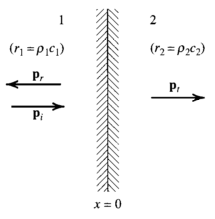
\includegraphics[width=0.35\textwidth]{Chapter-2/figs/reflectionWaves}
    \caption{Reflected Pressure Wave \cite{Kinsler1999}}
    \label{fig:reflectionWaves}
\end{figure}

The amount of energy reflected can be found by calculating the normal incidence reflection coefficient $R$
\begin{equation}
	\mathbf{R} = \frac{(r_n-r_1)+j x_n}{(r_n+r_1)+j x_n}
\end{equation}
However, any angle $\theta$ can be used by applying Snell's Law
\begin{equation}
	\frac{\sin \theta_1}{\sin \theta_2} = \frac{v_1}{v_2}
\end{equation}
which provides reflection coefficient generally as
\begin{equation}
	\mathbf{R} = \frac{(r_n-r_1/\cos \theta_i)+j x_n}{(r_n+r_1/\cos \theta_i)+j x_n}
\end{equation}

\subsection{Absorption}
The absorption coefficient is defined as
\begin{equation}
	\alpha = \sum_{i} \alpha_i
\end{equation}
where $\alpha_i$ represents each of the individual loss mechanisms calculated as if they were alone. The classical absorption coefficient $\alpha_c$ is the sum of the viscous and thermal absorption coefficients under the stokes assumption $\eta_B = 0$ and is defined as
\begin{equation}
	\alpha_c = \frac{\omega^2}{2\rho_0 c^3} \big(\frac{4}{3} + \frac{(\gamma - 1)\kappa}{c_P}\big)
\end{equation}

Mathematical formulation for calculating values is useful, however porous materials are complex by nature. Therefore, there are many formulas that are 'common sense' for acoustic engineers that are used in practice \cite{Bolt1944}. As a result, empirical equations for porous materials were developed by Biot \cite{Biot1962}.
The first experiments to calculate the absorption coefficient were carried out by Wallace C. Sabine in 1896 \cite{Bolt1944}. Sabine is credited with creating reverberation theory and the formula
\begin{equation}
	T = KV/\sum \alpha_j S_j
\end{equation}
The Eyring formula is the average absorption coefficient.
\begin{equation}
	\alpha = \sum \alpha_i S_i / \sum S_i
\end{equation}
The Eyring theory assumes that the energy in the room resumes uniform distribution after each set of incidences, and during the distribution after each set of incidences. All reverberation theory discussed is the energy lost at the walls. Rawlins \cite{Rawlins1983} corrected a small error made in formulation in \cite{Bolt1944}.

\section{Fiber Parameters}
Cellulose Acetate provided is a fibrous material and has some associated parameters that require definition.
\subsection{Total Denier}
Total Denier is the mass of a textile in grams per $9000$ meters. $1$ Denier is equivalent to $9000$ meters of fiber weighing $1$ gram.
\subsection{Denier per Filament (DPF)}
Denier per Filament (DPF) is defined as total denier divided by quantity of uniform filaments or 
\begin{equation}
	DPF = \frac{\text{Total Denier}}{\text{Quantity of uniform filaments}}
\end{equation}
\subsection{Fiber Cross Section}
Each fiber may have a different shape in its cross section. For experimental purposes in this paper, circular, X, Y and 8 legged cross sections were studied.  Table \ref{tab:crossSection} shows the fiber cross section.

\section{Chemical Relationships}
Cellulose Acetate is a polymer. A polymer is a chemical compound that is primarily composed of large quantities of similar repeating units. Polymers can be organic or inorganic, however, Cellulose Acetate is organic in structure \cite{Corsaro1990}.
A polymer's complex modulus is defined as:
\begin{equation}
	E^{*} = E' + iE''
\end{equation}
Where $E'$ is the storage modulus and $E''$ is the loss modulus.
The loss tangent is defined as:
\begin{equation}
	\tan{\delta} = E'' / E'
\end{equation}
The quantities $E''$ and $\tan{\delta}$ are of interest for absorption. Maximizing these parameters at a given frequency $f$ is the goal to maximize the absorption qualities of the material. It is important to note that with respect to frequency, $\tan{\delta}$ peaks at a higher temperature than $E''$ therefore making an optimal solution difficult to find as can be seen in Figure \ref{fig:tandelta}.
% Tan delta figure here
\begin{figure}[hbtp]
    \centering
    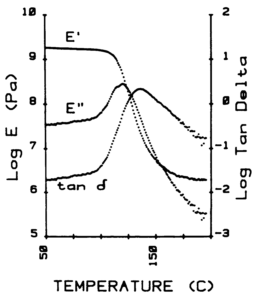
\includegraphics[width=0.4\textwidth]{Chapter-2/figs/tandelta}
    \caption{Typical Rheovibron data for polystyrene \cite{Corsaro1990}}
    \label{fig:tandelta}
\end{figure}

Temperature plays a role in the chemical reactions that result in porous absorption. The glass transition temperature of a polymer defined as $T_g$. The five regions of viscoelastic behavior can be found in Figure \ref{fig:viscoelasticregions}

% Viscoelastic Regions
\begin{figure}[hbtp]
    \centering
    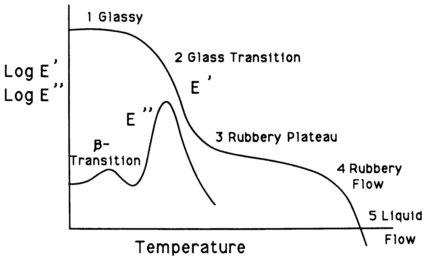
\includegraphics[width=0.7\textwidth]{Chapter-2/figs/viscoelasticregions}
    \caption{The five Viscoelastic Regions \cite{Corsaro1990}}
    \label{fig:viscoelasticregions}
\end{figure}

The key variables for damping are $T_g$, $E'$, $E''$, and $\tan{\delta}$

\section{Poroelastic Parameters}
Due to the complicated nature of absorption in porous materials, empirical methods have been developed \cite{Saint-Macary2006}. Viscoelastic porous materials are considered in a system of equations \cite{Shamaev2012}. Many of these methods rely on poroelastic parameters which have had much research in their identification \cite{Jaouen2008}. However, fibrous materials usually have no identifiable linear region, making these values difficult to measure \cite{Jaouen2008}. Fibers are usually layered causing materials to be anisotropic, however most materials are sufficiently homogenous for practical purposes and by only considering plane-wave propagation the isotropy requirement may be relaxed \cite{Delany1970}. Advances in technology are making it possible to run rather computationally intensive models to predict the properties of these kinds of waves in porous materials \cite{Mosanenzadeh2015}.\\
\indent The parameters can be broken down into fluid properties, structural properties, and fluid/structure interaction properties. This relies on the assumption made by Biot \cite{Biot1962} that sound traveling through porous material can be broken down into two categories; the fluid properties and the mechanical properties.

\subsection{Fluid Properties}
These properties relate to the behavior of the fluid as it travels through the porous object \cite{Sagartzazu2008}.\\
Volume Mass,
\begin{equation}
	\rho_0
\end{equation}
The Ratio of Specific Heats,
\begin{equation}
	\gamma = C_P/C_V
\end{equation}
Sound Velocity,
\begin{equation}
	c = \sqrt{\frac{\partial{\hat{p}}}{\partial \rho} (\rho_0, s_0)}
\end{equation}
where $c_0 = 331.5 \text{ m/s}$\\
Dynamic Viscosity,
\begin{equation}
	\eta = 1.72 x 10^{-5} \qquad \text{Pa $\centerdot$ s @ 0$^{\circ}$ C}
\end{equation}
Prandtl Number,
\begin{equation}
	P_r = \frac{\eta/\rho}{\kappa/\rho C_P} = \frac{\eta C_P}{\kappa}
\end{equation}
where the $P_r$ of air at $0^{\circ} \text{C}$ is equal to $0.708$
\subsection{Structural Properties}
These properties relate to the skeleton structure of the porous material \cite{Sagartzazu2008}
\begin{enumerate}
	\item Youngs Modulus, $E$
	\item Shear Modulus, $G$
	\item Poisson's Ratio, $\nu$
\end{enumerate}
\subsection{Fluid and Structural Interaction Properties}
These properties help define how the fluid and structural properties interface with one another \cite{Mosanenzadeh2015}.\\
Porosity,
\begin{equation}
	\phi = \frac{V_a}{V_t}
\end{equation}
Static Flow Resistivity,
\begin{equation}
	\sigma = \frac{8\eta}{\phi R^2}
\end{equation}
or,
\begin{equation}
	\sigma = E_1 \frac{7 \eta \alpha_{\infty}}{\phi R^2} (R_w)^{E_2} = E_1 \sigma' (R_w)^{E_2}
\end{equation}
Three non-acoustic properties:\\
Tortuosity,
\begin{equation}
	\alpha_{\infty} = \frac{\langle v_m^2 (N) \rangle _v}{v^2 (N_0)}
\end{equation}
The value of tortuosity is an intrinsic property of the porous frame that depends on the micro-geometry \cite{Mosanenzadeh2015}. Effective density of fluid $\rho$ is related to tortuosity by 
\begin{equation}
	\rho = \alpha_{\infty} \rho_0
\end{equation}
Viscous Characteristic Length,
\begin{equation}
	\Lambda = 2 \frac{\int_V v_i^2 (r) dV}{\int_A v_i^2 (r_w) dA}
\end{equation}
Thermal Characteristic Length,
\begin{equation}
	\Lambda' = \frac{2V_f}{A} = \frac{2l^3}{A_s(1-R_w)+(A_t-A_s)R_w}
\end{equation}
A fluid equivalent is based off of the Johnson-Champoux-Allard model.

\section{Empirical Models}
Due to complex expressions and the complex nature of porous materials, it is difficult to provide physical insight into the acoustic behavior of porous materials. It is also difficult to determine the dominate mechanism for sound absorption for a given material at a given frequency, $f$ \cite{Brennan2001}. There are currently two positions on prediction of acoustic properties of rigid-frame porous materials. One states that there are simple empirical expressions for noise control engineers to use and apply to predict the performance of porous material. Academic literature suggests relatively complicated expressions.\\
\indent The complicated expressions from academic literature often times require knowledge of many parameters of a material which is difficult to measure accurately. This also results in difficulty in determining which are the dominating physical traits of a material.\\
\indent Biot developed a model of mechanics of deformation and acoustic propagation in porous materials\cite{Biot1962}. Biot's model relies on the assumption that a porous material can be broken down into a fluid part and a solid part. This is the basis for many empirical models that have been based off of Biot's work. Generalized theory can be found in \cite{Biot1962a}. Dazel considers a porous elastic matrix as a fluid-saturated and statistically isotropic material. This work brings forth a general correspondence principle by which known results for elastic media may be immediately extended to the case of viscoelasticity by substituting operators for the elastic coefficient. Many authors have extended this work to generalize his theory \cite{Dazel2007} \cite{Albers2012}. Some newer equations have resulted in improved performance of the model in the lower frequency range \cite{Allard1992}.\\
\indent However, some authors still would like to reduce the complicated nature of the equations and bridge the gap between the complex expressions presented in academic literature and simplified expressions practically used  \cite{Brennan2001}. Brennan takes note that the effects of thermal losses are negligible in most situations and an upper bound on the thermal losses can be derived.\\
\indent A rigid local reacting porous material has two characteristics that describe its behavior. These are the acoustic wave number $k_c$ and the characteristic acoustic impedance $Z_c$.
\begin{equation}
	k_c = \omega \Big(\frac{\rho_e}{B_e}\Big)^{\frac{1}{2}}
\end{equation}
\begin{equation}
	Z_c = (\rho_e B_e)^{\frac{1}{2}}
\end{equation}
where $\rho_e$ and $B_e$ are the effective density and bulk modulus of the fluid contained within the porous material respectively.\\
\indent To approximate $\phi_e$ and $B_e$ the following expressions have been derived \cite{Brennan2001}
\begin{equation}
	\rho_e = \rho_0 \alpha_{\infty} \bigg( 1 + j \frac{\eta \phi}{\rho_0 \alpha_{\infty} k_0 \omega} \Big( 1 - j \frac{4\rho_0 \alpha_{\infty}^2 k_0^2 \omega}{\eta \phi^2 \Lambda^2} \Big) \bigg)
\end{equation}
\begin{equation}
		B_e = \frac{\gamma P}{\gamma - (\gamma - 1) \bigg( 1 + j \frac{\eta \phi}{\rho_0 Pr k'_0 \omega} \Big( 1 - j \frac{4 \rho_0 Pr k'_0 \omega}{\eta \phi^2 \Lambda'^2} \Big) ^{\frac{1}{2}} \bigg)^{-1}}
\end{equation}

Delany and Bazley's empirical model estimates the value of the propagation constant $jk_C$ and characteristic impedance $Z_C$ as a function of material flow resistivity. This model assumes that the material is fibrous and that the fibers are uniformly distributed. However, this only works well in a specific frequency range \cite{Sagartzazu2008}.
% these are emprical equations from Delaney and Bazley
\begin{equation}
	\rho_1/\rho = (\vert \rho_1 \vert / \rho) \exp {j \phi} = \mathbf{kW}/\rho \omega
\end{equation}
\begin{equation}
	\kappa / \gamma \mathbf{P} = (\vert \kappa \vert / \gamma \mathbf{P}) \exp {j \theta} = \omega W/k \rho c^2
\end{equation}
\begin{equation}
	W = \rho c [1 + 0.0571 X^{-0.754} - j0.087 X^{-0.732}]
\end{equation}
\begin{equation}
	k = (\omega/c)[(1+0.0978X^{-0.700}) - j0.189X^{-0.595}]
\end{equation}
where the frequency parameter is
\begin{equation}
	X = \rho f/R_1
\end{equation}

Delaney and Bazley suggest bounds for the validity of the empirical equation on the parameter $X$ as follows:
\begin{equation}
	0.01 < X < 1.0
\end{equation}

The Mechel-V�r model is a more refined adjustment than the Delany and Bazley model. It differentiates two families of absorption materials, and two areas for normalized adimensional parameters that are called the normalized frequency parameter, $E = \rho_0 f / \sigma$

\begin{equation}
	Z_C = \rho_0 c(1 + b' E^{-\beta'} - jb'' E^{-\beta''})
\end{equation}
\begin{equation}
	\Gamma_c = \frac{\omega}{c}[a' E^{-\alpha'} + j(1 + \alpha'' E^{-\alpha''}) ]
\end{equation}
that is
\begin{equation}
	k_C = -j \frac{\omega}{c} [a' E^{-\alpha'} + j(1 + \alpha'' E^{-\alpha''})]
\end{equation}
This model is even more accurate at lower frequencies than the Delany-Bazley model.\\
\indent Another recent empirical model that has been developed is the Allard-Champoux model. This model assumes that the thermal effects depend on the frequency. This model currently shows better results at low frequencies than all previous models. This model defines dynamic density and the compressibility modulus as follows:
\begin{equation}
	\rho(\omega) = \rho_0 \Big[1 - j \Big( \frac{\sigma}{\rho_0 \omega} \Big) G_1 \Big( \frac{\rho_0 \omega}{\sigma} \Big) \Big]
\end{equation}
\begin{equation}
	K(\omega) = \gamma P_0 \Big( \gamma - \frac{\gamma - 1}{1 - (\frac{j}{4 P_r}) (\frac{\sigma}{\rho_0 \omega}) G_2 (\frac{\rho_0 \omega}{\sigma})} \Big)^{-1}
\end{equation}
where $G_1(\rho_0 \omega/\sigma)$ and $G_2 (\rho_0 \omega/\sigma)$ are defined as
\begin{equation}
	G_1 \Big( \rho_0 \omega/\sigma \Big) = \sqrt{1 + \frac{j}{2} \bigg( \rho_0 \omega/\sigma \bigg)}
\end{equation}
\begin{equation}
	G_2 \Big( \frac{\rho_0 \omega}{\sigma} \Big) = G_1 \Big( \frac{\rho_0 \omega}{\sigma} \Big) \Big( 4 P_r \Big( \frac{\rho_0 \omega}{\sigma} \Big) \Big)
\end{equation}
where $P_0$ is the balance pressure.

With many different models available, Figure \ref{fig:empiricalcomparisons} shows that many of the empirical modeling techniques adherer to experimental data well.
% Empirical Comparisons
\begin{figure}[hbtp]
    \centering
    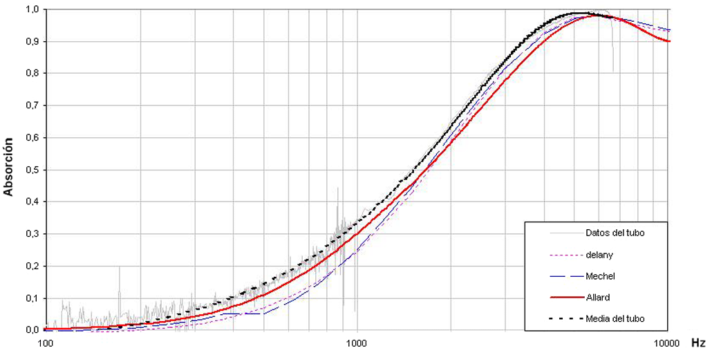
\includegraphics[width=1\textwidth]{Chapter-2/figs/empiricalcomparisons}
    \caption{Comparison of Empirical Approximations on wool type material \cite{Sagartzazu2008}}
    \label{fig:empiricalcomparisons}
\end{figure}
\clearpage

Many authors have taken the results of the work by Biot et al. to use in their in their own research applications. Topics range from Helmholtz resonators \cite{Boutin2013}, to finite-element modeling \cite{Atalla2001}, \cite{Rumpler2012}, \cite{Kook2014}, to the scattering effect of non-porous materials \cite{Velea2001}, to Rayleigh attenuation \cite{Bouhedja2011}, and to various other acoustic materials \cite{Voronina1998} \cite{Voronina1999} \cite{Biot1934}.

\section{Measurement Techniques}
Measurement of acoustic parameters is of interest \cite{Gayathri2013}, \cite{Horoshenkov2001}. The empirical models rely on the ability to accurately measure parameters about the test sample. Many techniques have been developed to obtain these values.

\subsection{Flow Resistance}
The flow resistance of a material plays a large role in an open cell porous material's ability to interface with sound \cite{Ingard1985}. Flow resistance can be measured using a two-channel analyzer. The normalized flow resistance is the absolute value of the imaginary part of the pressure ratio, or $\theta = \vert \operatorname{Im}(p_1/p_3) \vert$. At low frequencies the flow reactance is small compared to the resistance and can be approximated by $\theta = \vert p_1/p_3 \vert$.
Normalized flow reactance is as follows
\begin{equation}
	\chi = (-1)^{n-1} \operatorname{Re}(p_1/p_3)
\end{equation}

Other calculations relying on the Kozeny number \cite{Lambert1984} or reflected waves \cite{Sebaa2005} to find static flow resistance also are valid. Figure \ref{fig:flowresistancemeasurement} shows a device used by Bies.

% Flow Resistance Measurement Device
\begin{figure}[hbtp]
    \centering
    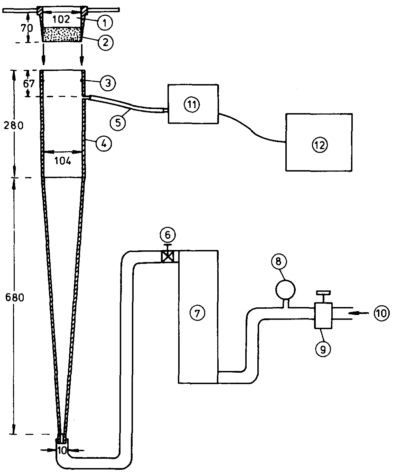
\includegraphics[width=0.45\textwidth]{Chapter-2/figs/flowresistancemeasurement}
    \caption{Flow Resistance Measurement Device \cite{Bies1980}}
    \label{fig:flowresistancemeasurement}
\end{figure}

\subsection{Tortuosity}
Allard developed a technique for the measurement of tortuosity in air saturated open cell porous sound absorbing materials. It is noted that it is difficult to obtain the measurement for some materials without damaging the sample material \cite{Allard1994}.

\subsection{Porosity}
% Measurement - Porosity
Porosity is defined as the volume fraction of air contained in a material. This technique is based on the ideal gas law. \cite{Champoux1991}
\begin{equation}
	\phi = V_a/V_t
\end{equation}
where $V_a$ is the air filled volume and $V_t$ is the total volume. The total volume of air in the measurement chamber is $V' = V_0 + V_a$ where $V_0$ is the residual volume in the sample chamber outside of the sample. Figure \ref{fig:porositychamber} shows this test set up.
% Porosity chamber measurement figure !
\begin{figure}[hbtp]
    \centering
    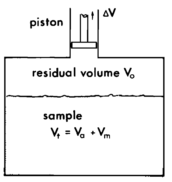
\includegraphics[width=0.4\textwidth]{Chapter-2/figs/porositychamber}
    \caption{Porosity Measurement Chamber}
    \label{fig:porositychamber}
\end{figure}
Then $V_a$ is calculated by
\begin{equation}
	V' = -[(P_0 + \Delta P')/ \Delta P'] \Delta V
\end{equation}
and air content is then
\begin{equation}
	V_a = V' - V_0
\end{equation}

To help determine the internal pore surface area per unit area of a solid, \cite{Leclaire1998} developed a technique for integrating the water extraction curve. This method works well for acoustic type materials to determine the specific area needed in previous calculations.

\subsection{Impedance}
Impedance measurement of porous materials is an important topic \cite{McGrath1952}. There are techniques developed by Allard for in situ measurement of acoustic surface impedance, which can provide valuable information when manufacturing acoustic absorption materials. A technique using two-microphones above the surface of which impedance is measured is detailed in \cite{Allard1989}, and again in \cite{Allard2003} for porous materials.

\subsection{Reflection Coefficients}

Tamara developed the technique for measuring reflection coefficient at oblique angles \cite{Tamura1990} and continued on in \cite{Tamura1995} with experimental results. The basic principle relies on decomposing spherical waves into plane waves by spatial Fourier transform. Decomposing spherical waves into plane waves is done by
\begin{equation}
	P(k_x,k_y,k_z) = \int \int_{-\infty}^{\infty} p(x,y,z_j) \exp{-i(k_x x + k_y y)} dx dy
\end{equation}
\begin{figure}[hbtp]
    \centering
    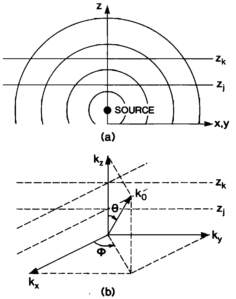
\includegraphics[width=0.5\textwidth]{Chapter-2/figs/sphericaltoplanewaves}
    \caption{Decompose Spherical Waves into Plane Waves}
    \label{fig:sphericaltoplanewaves}
\end{figure}

Solving this for incident and reflected pressure-wave components in the x-y plane we get the following expressions for $P_i$ and $P_r$
\begin{equation}
	P_i(k_x,k_y,0)  = \frac{P(k_x,k_y,z_1)\exp{i k_z z_2} - P(k_x,k_y,z_2) \exp{i k_z z_1}}{2 i \sin{k_z (z_2 - z_1)}}
\end{equation}
\begin{equation}
	P_r(k_x,k_y,0) = \frac{P(k_x,k_y,z_2)\exp{-i k_z z_2} - P(k_x,k_y,z_1) \exp{-i k_z z_1}}{2 i \sin{k_z(z_2 - z_1)}}
\end{equation}
where coefficient of reflection $C_r$ is defined as the ratio between the reflected and incident pressure waves
\begin{equation}
	C_r(k_x,k_y) = P_r(k_x,k_y,0) / P_i(k_x,k_y,0)
\end{equation}

This theory has been modeled using the reflection coefficient of absorbing materials measured from an impedance tube for normal sound incidence \cite{Lanoye2006}. The Tamara method can determine the angle dependency of the surface impedance and the absorption coefficient. The Tamura technique measures sound pressure in two planes parallel to the surface of interest, and a 2d Fourier transformation is used to calculate the angle dependent surface impedance.

In a standing wave tube the sound pressure at a distance $x$ from the rigid ending is given by
\begin{equation}
	p(x,t,\omega) = A(\exp{ikx}+\exp{-ikx})\exp{-i\omega t}
\end{equation}
and the particle velocity at the same distance is defined by
\begin{equation}
	u(x,t,\omega) = \frac{1}{i\omega \rho_0} \frac{\partial p(x,t,\omega)}{\partial x} = \frac{A}{\rho_0 c} (\exp{ikx} - \exp{-ikx}) \exp{-i \omega t}
\end{equation}
These values are calculated in real time using a well calibrated velocity-pressure transducer. From this knowledge the value of the surface impedance can be calculated for normal to slightly oblique incidence. Figure \ref{fig:reflectionWavesrelatedAbsorption} shows that pressure reflection coefficient is inversely proportional to absorption coefficient.
% Reflected Waves figure 2
\begin{figure}[hbtp]
    \centering
    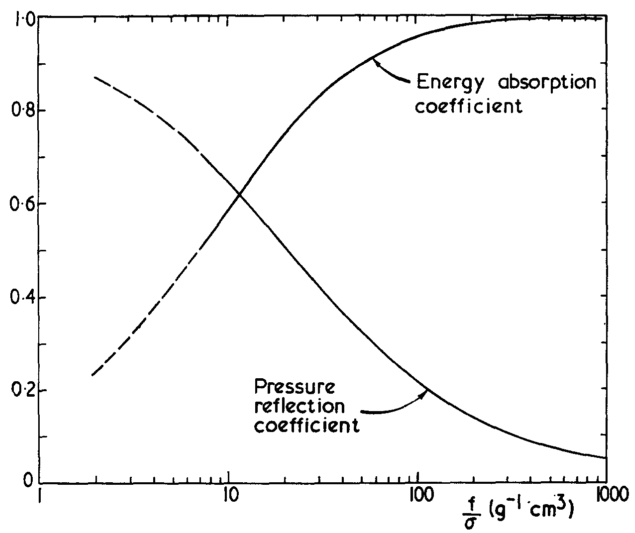
\includegraphics[width=0.7\textwidth]{Chapter-2/figs/reflectionWavesrelatedAbsorption}
    \caption{Reflected Pressure Coefficient Relation to Absorption \cite{Delany1970}}
    \label{fig:reflectionWavesrelatedAbsorption}
\end{figure}

\section{Impedance Tube Method Definition}

Referencing \cite{Kjaer2011} includes detailed information on how the Impedance tube system is able to calculate its value for absorption coefficient $\alpha$. Figures \ref{fig:impedancetube2} and \ref{fig:impedancetube3} show the system configuration.

% Testing set up 1
\begin{figure}[hbtp]
    \centering
    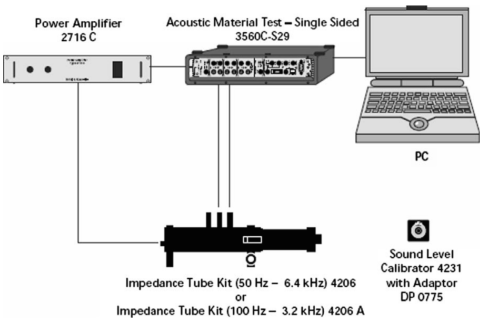
\includegraphics[width=0.95\textwidth]{Chapter-2/figs/impedancetube2}
    \caption{Impedance Tube Testing Set up \cite{Ersoy2009}}
    \label{fig:impedancetube2}
\end{figure}

% Impedance Tube Method
\begin{figure}[hbtp]
    \centering
    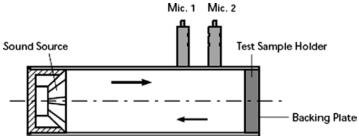
\includegraphics[width=0.75\textwidth]{Chapter-2/figs/impedancetube3}
    \caption{Impedance Tube Method \cite{Ersoy2009}}
    \label{fig:impedancetube3}
\end{figure}

The two-microphone system functions by decomposing the incident wave generated by the sound source into its incident and reflected components. From this information, the complex reflection coefficient $R$ is found by:
\begin{equation}
	R = \Bigg( \frac{H_1 - H_i}{H_r - H_1} \Bigg) \exp{j 2 k (l + s)}
\end{equation}
where $k$ is the wave number, $l$ is the distance from the first microphone to the front of the sample, $s$ is the distance between the two microphones, and $H$ are frequency response functions. $H_i$ corresponds to the incident component, $H_r$ corresponds to the reflected component and $H_1$ corresponds to the sample.

From the complex reflection coefficient, the system is able to find the normalized impedance ratio $(z/\rho c)$and absorption coefficient $\alpha$ by the following equations.

%normalied impedance ratio
\begin{equation}
	\frac{z}{\rho c} = \frac{1+R}{1-R}
\end{equation}
% sound absorption coefficient
\begin{equation}
	\alpha = 1 - \vert R \vert ^2
\end{equation}
It should be noted that two-microphone theory assumes plane-wave propagation, no mean flow, and no losses due to absorption at the tube wall. 

\subsection{Microphone Calibrations}
In order for the system to accurately find the frequency response functions $H$, each microphone must be properly calibrated by a calibration factor $H_C$ found by:
\begin{equation}
	H_C = \vert H_C \vert \exp{j \phi_C}
\end{equation}
where
\begin{equation}
	H_c = \sqrt{\vert H_{C1}\vert \vert H_{C2}\vert}
\end{equation}
\begin{equation}
	\phi_C = \frac{1}{2} (\phi_1 + \phi_2)
\end{equation}
where $\phi_1$ and $\phi_2$ are the phase of the calibration frequency response $H_C1$ and $H_C2$ respectively.
Applying this correction factor to $H_1$ yeilds
\begin{equation}
	H_1 = \frac{H}{H_C} = \vert H_1 \vert \exp{j \phi_h}
\end{equation}
where
\begin{equation}
	\phi_h = \phi - \phi_C
\end{equation}
Once this calibration is applied, the value $H_1$ is used to determine the acoustic properties of the test sample.

\subsection{Working Frequency Range}
The theoretical impedance tube system would span a relatively large frequency range, however in practice the working frequency range is much smaller. The working frequency range is defined by
\begin{equation}
	f_l < f < f_u
\end{equation}
The lower working frequency $f_l$ is limited. \cite{ISO1998}.
\begin{itemize}
	\item The $f$ resolution of the analysis system
	\item The $f$ response of the loudspeaker
	\item The spacing between the microphones
\end{itemize}
The upper working frequency $f_u$ is chosen to avoid the occurrence of non-plane wave mode propagation and to assure accurate phase detection \cite{Kjaer2011}. Various standards provide guidelines for the physical concerns of the system. \cite{ASTM1990}, \cite{ASTM2011}.

In order to maintain plane wave propagation, the upper frequency limit is defined as:
\begin{equation}
	f_u < K c / d \qquad \text{or} \qquad d < K c / f_u
\end{equation}
where $f_u$ is the upper frequency limit, $c$ is the speed of sound in the tube, $d$ is the diameter of the tube, and $K = 0.586$.

A large spacing between the microphones enhances accuracy of the measurements, however the spacing must be less than the shortest half-wavelength of interest.
\begin{equation}
	s << c / 2 f_u
\end{equation}
where $s$ is microphone spacing. It is recommended that s be $80\%$ of $c / 2 f_u$.

The length of the tube should be sufficiently long enough as to allow plane waves to fully develop before reaching the microphones and test specimen. A recommended minimum is three tube diameters between the sound source and the nearest microphone.

The specimens location relative to the closest microphone is ideally at a minimum, however the surface characteristics of the sample play a role. This distance can be modified as follows.
\begin{itemize}
	\item Flat Surface
	The closest microphone can be within one-half of the tube diameter.
	\item Nonhomogenous Surface
	The closet microphone can be at least one tube diameter in order to suppress higher order modes resultant of the non homogenous surface of the sample.
	\item Asymmetrical Surface
	The closest microphone can be at least two tube diameters to suppress higher order modes resultant.
\end{itemize}

For the Impedance Tube system used in the experiments in this paper, Table \ref{tab:workingfreq} shows the appropriate associated values.

% Landscape page of Samples from Eastman Chemical Company
\newgeometry{margin=1in,lmargin=1.25in,footskip=\chapterfootskip, includehead, includefoot}
    %\thispagestyle{lscape}
    %\pagestyle{lscape}
    \thispagestyle{lscapedplain}
    \begin{landscape}
	\begin{table}
    \caption{Working Frequencies of Impedance Tube}
    \label{tab:workingfreq}
    \begin{center}
    \begin{tabular}{lcl}
    \toprule
    Parameter & Large Tube Wide Spacing & Small Tube\\
    \midrule
    Tube Diameter (mm) & 100 & 29\\
    Microphone Spacing (mm) & 100 & 20\\
    Distance from Sample to Mic B (mm) & 100 & 35\\
    Distance from Source to Mic A (mm) & 100 & 370\\
    Provided Lower Frequency Limit (Hz) & 50 & 500\\
    Provided Upper Frequency Limit (Hz) & 1600 & 6400\\
    Calculated Lower Frequency Limit (Hz) & 34.3 & 171.5\\
    Calculated Upper Frequency Limit (Hz) (Based on Diameter) & 2010 & 6931\\
    Calculated Upper Frequency Limit (Hz) (Based on Microphone Spacing) & 1372 & 6860\\
    \bottomrule
    \end{tabular}
    \end{center}
	\end{table}
    \end{landscape}
    %\newgeometry{margin=1in,lmargin=1.25in,footskip=\chapterfootskip, includehead, includefoot,landscape=false}
    \restoregeometry
    \pagestyle{fancy}
    \thispagestyle{fancy}
\newgeometry{margin=1in,lmargin=1.25in,footskip=\chapterfootskip, includehead, includefoot}



